Concurrent stochastic multi-player games (CSGs) \cite{Kwiatkowska2019,Kwiatkowska2020} is an extension of Probabilistic Automata (PA) PA \cite{ref27}  where the formalism is based on the idea that players make choices concurrently in each state and then transition simultaneously. In CSGs, each player controls one or more modules, and the actions that label commands within a player's modules must only be used by that specific player. 

To express the coalition game, we rely on PRISM \cite{Kwiatkowskaprism2011}. The PRISM model is composed of a set of modules that can synchronize. A set of variables and commands characterizes each module. The variable's valuations represent the state of the module \cmt{represented by \emath{S}}. A set of commands is used to describe the behavior of each module (i.e., transitions). A command takes the form: $ [a_{1}, \ldots, a_{n}] g \rightarrow \lambda_{1}: u_{1} + \ldots+ \lambda_{n}: u_{n} $ or, \emath{[a_{1}, \ldots, a_{n}] g \rightarrow u}, which means, for actions \emath{a_{i}} \cmt{(\emath{a_{i} \in A})} if the guard \quot{\emath{g}} is true, then, an update \quot{\emath{u_{i}}} is enabled with a probability \quot{\emath{\lambda_{i}}}. A guard is a logical proposition consisting of variable evaluation and propositional logic operators. The update \quot{\emath{u_{i}}} is an evaluation of variables expressed as a conjunction of assignments: \emath{v_{i}'=val_{i}+\ldots+v_{n}'=val_{n}} where \quot{\emath{v_{i}}} \cmt{\emath{\in V}, such that V is a set local and global variable} are local variables and \emath{val_{i}} are values evaluated via expressions denoted by \quot{\emath{\theta}} such that \emath{ \theta: V \rightarrow \mathbb{D}}, \cmt{\emath{\mathbb{D}} is the domain variables}. 

CSGs are augmented with reward structures \cite{Kwiatkowska2019,Kwiatkowska2020}  as \emath{r_{A} : S \times A \longrightarrow \mathbb{R}} is an action reward function which assigns each state (\emath{s\in S}) and action (\emath{a \in A}) tuple pair to a real value that is accumulated when the action tuple is selected in the state and \emath{r_{s} : S \longrightarrow \mathbb{R}}  is a state reward function which assigns each state to a real value that is accumulated when the state is reached.


The properties related to CSGs are expressed in the temporal logic rPATL \cite{hutchisonautomatic2012} (short for reward Probabilistic Alternating Temporal Logic). The property grammar is based on CTL \cite{baierprinciples2008} extended with coalition operator \emathtt{\langle\langle C\rangle\rangle} of ATL \cite{Alur2002} and probabilistic operator \emathtt{P} of PCTL \cite{hanssonlogic1994}. For instance, for the following property expressed in natural language: \quot{\emph{Players 1 and 2 have a strategy to ensure that the probability of system failure occurring within 100 rounds is less than 0.001, regardless of the strategies of attacks}} is expressed in rPATL as: \emathtt{\langle\langle 1,2\rangle\rangle P_{<0.001} [ F \ (fail  \ \& \ rounds =100)]}. Here, \quot{\emathtt{fail}} is the label that refers to the system failure states. Concerning rewards structure, the property expressed in natural language: \quot{\emph{What is the reward r within 100 rounds to reach \quot{\emathtt{fail}} for both Players 1 and 2 for a selected strategy ?}} is expressed in rPATL as \emathtt{\langle\langle 1,2\rangle\rangle R=? [  F \ (fail  \ \& \ rounds =100)] }

\begin{example}
\label{exp:csg:architecture}   
Consider the CSG shown in \fig{fig:even:odds} in \cite{BAOUYA2024101161}, which corresponds to two players repeatedly performing a scheduled read and write operation. Transitions are labeled with actions where \emath{A = (r_{1}r_{2}), (w_{1}w_{2}), (w_{2}r_{1}), (r_{2}w_{2}), (reset_{1} reset_{2}).}The CSG starts in state \quot{s0}, and states \quot{s1}, \quot{s2}, and \quot{s3} are labeled with atomic propositions corresponding to a player winning. Each player is involved by writing and reading operations.
%\tikzset{every picture/.style={ scale=0.95,line width=0.2pt}} %set default line width to     
\noindent
\begin{figure}[!htb]
    \centering
    %


\tikzset{every picture/.style={line width=1.05pt}} %set default line width to 0.75pt        

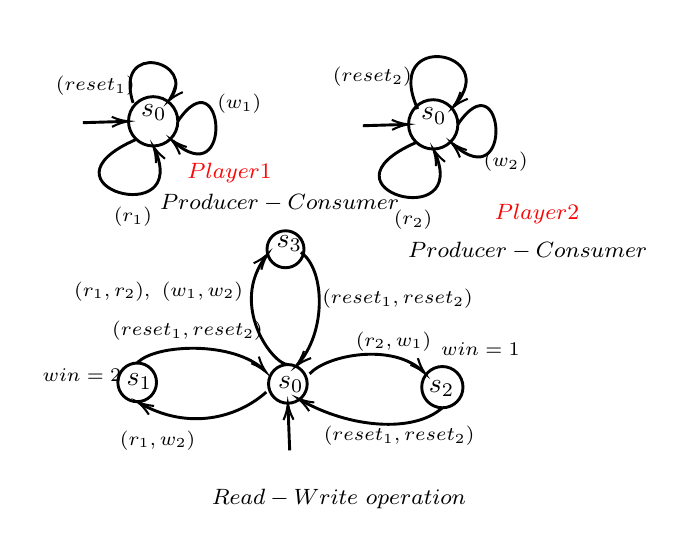
\begin{tikzpicture}[x=0.55pt,y=0.55pt,yscale=-1,xscale=1]
%uncomment if require: \path (0,300); %set diagram left start at 0, and has height of 300

%Shape: Circle [id:dp8314413576675287] 
\draw   (149.6,126.85) .. controls (149.6,120.14) and (155.04,114.7) .. (161.75,114.7) .. controls (168.46,114.7) and (173.9,120.14) .. (173.9,126.85) .. controls (173.9,133.56) and (168.46,139) .. (161.75,139) .. controls (155.04,139) and (149.6,133.56) .. (149.6,126.85) -- cycle ;
%Shape: Circle [id:dp7772472429687135] 
\draw   (150.6,215.3) .. controls (150.6,208.29) and (156.29,202.6) .. (163.3,202.6) .. controls (170.31,202.6) and (176,208.29) .. (176,215.3) .. controls (176,222.31) and (170.31,228) .. (163.3,228) .. controls (156.29,228) and (150.6,222.31) .. (150.6,215.3) -- cycle ;
%Shape: Circle [id:dp8090258776189614] 
\draw   (251.25,217.45) .. controls (251.25,209.97) and (257.32,203.9) .. (264.8,203.9) .. controls (272.28,203.9) and (278.35,209.97) .. (278.35,217.45) .. controls (278.35,224.93) and (272.28,231) .. (264.8,231) .. controls (257.32,231) and (251.25,224.93) .. (251.25,217.45) -- cycle ;
%Shape: Circle [id:dp44457702069517324] 
\draw   (51.6,214.3) .. controls (51.6,207.29) and (57.29,201.6) .. (64.3,201.6) .. controls (71.31,201.6) and (77,207.29) .. (77,214.3) .. controls (77,221.31) and (71.31,227) .. (64.3,227) .. controls (57.29,227) and (51.6,221.31) .. (51.6,214.3) -- cycle ;
%Curve Lines [id:da7159034648648847] 
\draw    (163.3,202.6) .. controls (153.45,202.6) and (124.2,163.79) .. (149.12,131.19) ;
\draw [shift={(150.3,129.7)}, rotate = 129.37] [color={rgb, 255:red, 0; green, 0; blue, 0 }  ][line width=0.75]    (10.93,-3.29) .. controls (6.95,-1.4) and (3.31,-0.3) .. (0,0) .. controls (3.31,0.3) and (6.95,1.4) .. (10.93,3.29)   ;
%Curve Lines [id:da856509401174204] 
\draw    (171.9,128.85) .. controls (188.17,140.51) and (188.49,182.04) .. (169.68,202.52) ;
\draw [shift={(168.5,203.75)}, rotate = 315] [color={rgb, 255:red, 0; green, 0; blue, 0 }  ][line width=0.75]    (10.93,-3.29) .. controls (6.95,-1.4) and (3.31,-0.3) .. (0,0) .. controls (3.31,0.3) and (6.95,1.4) .. (10.93,3.29)   ;
%Curve Lines [id:da5490799952546435] 
\draw    (149.1,220.7) .. controls (130.39,237.44) and (98.09,246.43) .. (65.78,227.87) ;
\draw [shift={(64.3,227)}, rotate = 30.99] [color={rgb, 255:red, 0; green, 0; blue, 0 }  ][line width=0.75]    (10.93,-3.29) .. controls (6.95,-1.4) and (3.31,-0.3) .. (0,0) .. controls (3.31,0.3) and (6.95,1.4) .. (10.93,3.29)   ;
%Curve Lines [id:da32420249193131656] 
\draw    (64.3,201.6) .. controls (75.86,188.96) and (127.96,186.78) .. (147.92,206.47) ;
\draw [shift={(149.1,207.7)}, rotate = 227.86] [color={rgb, 255:red, 0; green, 0; blue, 0 }  ][line width=0.75]    (10.93,-3.29) .. controls (6.95,-1.4) and (3.31,-0.3) .. (0,0) .. controls (3.31,0.3) and (6.95,1.4) .. (10.93,3.29)   ;
%Curve Lines [id:da5468630552582512] 
\draw    (177.6,208.7) .. controls (189.16,196.06) and (232.81,188.03) .. (252.43,207.47) ;
\draw [shift={(253.6,208.7)}, rotate = 227.86] [color={rgb, 255:red, 0; green, 0; blue, 0 }  ][line width=0.75]    (10.93,-3.29) .. controls (6.95,-1.4) and (3.31,-0.3) .. (0,0) .. controls (3.31,0.3) and (6.95,1.4) .. (10.93,3.29)   ;
%Curve Lines [id:da7774551676749778] 
\draw    (264.8,231) .. controls (246.09,247.75) and (203.7,244.5) .. (171.08,225.58) ;
\draw [shift={(169.6,224.7)}, rotate = 30.99] [color={rgb, 255:red, 0; green, 0; blue, 0 }  ][line width=0.75]    (10.93,-3.29) .. controls (6.95,-1.4) and (3.31,-0.3) .. (0,0) .. controls (3.31,0.3) and (6.95,1.4) .. (10.93,3.29)   ;
%Straight Lines [id:da9977682076817751] 
\draw    (164.5,259) -- (163.38,230) ;
\draw [shift={(163.3,228)}, rotate = 87.78] [color={rgb, 255:red, 0; green, 0; blue, 0 }  ][line width=0.75]    (10.93,-3.29) .. controls (6.95,-1.4) and (3.31,-0.3) .. (0,0) .. controls (3.31,0.3) and (6.95,1.4) .. (10.93,3.29)   ;
%Shape: Circle [id:dp1467498401619306] 
\draw   (242.6,44.8) .. controls (242.6,35.85) and (249.85,28.6) .. (258.8,28.6) .. controls (267.75,28.6) and (275,35.85) .. (275,44.8) .. controls (275,53.75) and (267.75,61) .. (258.8,61) .. controls (249.85,61) and (242.6,53.75) .. (242.6,44.8) -- cycle ;

%Curve Lines [id:da20144538683966495] 
\draw    (248.6,34.7) .. controls (224.84,-17.77) and (304.97,-3.59) .. (272.62,32.6) ;
\draw [shift={(271.6,33.7)}, rotate = 313.41] [color={rgb, 255:red, 0; green, 0; blue, 0 }  ][line width=0.75]    (10.93,-3.29) .. controls (6.95,-1.4) and (3.31,-0.3) .. (0,0) .. controls (3.31,0.3) and (6.95,1.4) .. (10.93,3.29)   ;
%Curve Lines [id:da01826233197981253] 
\draw    (275,44.8) .. controls (305.29,0.15) and (312.46,93.79) .. (271.85,57.83) ;
\draw [shift={(270.6,56.7)}, rotate = 42.88] [color={rgb, 255:red, 0; green, 0; blue, 0 }  ][line width=0.75]    (10.93,-3.29) .. controls (6.95,-1.4) and (3.31,-0.3) .. (0,0) .. controls (3.31,0.3) and (6.95,1.4) .. (10.93,3.29)   ;
%Curve Lines [id:da45337553182486945] 
\draw    (247.6,56.7) .. controls (177.31,87.39) and (284.42,117.1) .. (259.59,62.68) ;
\draw [shift={(258.8,61)}, rotate = 63.88] [color={rgb, 255:red, 0; green, 0; blue, 0 }  ][line width=0.75]    (10.93,-3.29) .. controls (6.95,-1.4) and (3.31,-0.3) .. (0,0) .. controls (3.31,0.3) and (6.95,1.4) .. (10.93,3.29)   ;
%Straight Lines [id:da9810106035384246] 
\draw    (212.6,45.7) -- (240.6,44.86) ;
\draw [shift={(242.6,44.8)}, rotate = 178.28] [color={rgb, 255:red, 0; green, 0; blue, 0 }  ][line width=0.75]    (10.93,-3.29) .. controls (6.95,-1.4) and (3.31,-0.3) .. (0,0) .. controls (3.31,0.3) and (6.95,1.4) .. (10.93,3.29)   ;
%Shape: Circle [id:dp6710432398464078] 
\draw   (58.6,42.8) .. controls (58.6,33.85) and (65.85,26.6) .. (74.8,26.6) .. controls (83.75,26.6) and (91,33.85) .. (91,42.8) .. controls (91,51.75) and (83.75,59) .. (74.8,59) .. controls (65.85,59) and (58.6,51.75) .. (58.6,42.8) -- cycle ;

%Curve Lines [id:da7849548233918409] 
\draw    (61.6,30.7) .. controls (48.27,-11.15) and (104.67,3.38) .. (85.85,28.17) ;
\draw [shift={(84.6,29.7)}, rotate = 311.08] [color={rgb, 255:red, 0; green, 0; blue, 0 }  ][line width=0.75]    (10.93,-3.29) .. controls (6.95,-1.4) and (3.31,-0.3) .. (0,0) .. controls (3.31,0.3) and (6.95,1.4) .. (10.93,3.29)   ;
%Curve Lines [id:da3143750611128635] 
\draw    (91,42.8) .. controls (121.29,-1.85) and (128.46,91.79) .. (87.85,55.83) ;
\draw [shift={(86.6,54.7)}, rotate = 42.88] [color={rgb, 255:red, 0; green, 0; blue, 0 }  ][line width=0.75]    (10.93,-3.29) .. controls (6.95,-1.4) and (3.31,-0.3) .. (0,0) .. controls (3.31,0.3) and (6.95,1.4) .. (10.93,3.29)   ;
%Curve Lines [id:da830110688853805] 
\draw    (63.6,54.7) .. controls (-6.69,85.39) and (100.42,115.1) .. (75.59,60.68) ;
\draw [shift={(74.8,59)}, rotate = 63.88] [color={rgb, 255:red, 0; green, 0; blue, 0 }  ][line width=0.75]    (10.93,-3.29) .. controls (6.95,-1.4) and (3.31,-0.3) .. (0,0) .. controls (3.31,0.3) and (6.95,1.4) .. (10.93,3.29)   ;
%Straight Lines [id:da9076150365855119] 
\draw    (28.6,43.7) -- (56.6,42.86) ;
\draw [shift={(58.6,42.8)}, rotate = 178.28] [color={rgb, 255:red, 0; green, 0; blue, 0 }  ][line width=0.75]    (10.93,-3.29) .. controls (6.95,-1.4) and (3.31,-0.3) .. (0,0) .. controls (3.31,0.3) and (6.95,1.4) .. (10.93,3.29)   ;


% Text Node
\draw (297,95) node [anchor=north west][inner sep=0.75pt]  [font=\footnotesize,color={rgb, 255:red, 247; green, 6; blue, 6 }  ,opacity=1 ]  {$Player2$};
% Text Node
\draw (77,88) node [anchor=north west][inner sep=0.75pt]  [font=\footnotesize]  {$Producer-Consumer$};
% Text Node
\draw (8.6,10.7) node [anchor=north west][inner sep=0.75pt]  [font=\scriptsize]  {$( reset_{1})$};
% Text Node
\draw (114.6,22.7) node [anchor=north west][inner sep=0.75pt]  [font=\scriptsize]  {$( w_{1})$};
% Text Node
\draw (46.6,96.7) node [anchor=north west][inner sep=0.75pt]  [font=\scriptsize]  {$( r_{1})$};
% Text Node
\draw (95,68) node [anchor=north west][inner sep=0.75pt]  [font=\footnotesize,color={rgb, 255:red, 252; green, 6; blue, 6 }  ,opacity=1 ]  {$Player1$};
% Text Node
\draw (240,120) node [anchor=north west][inner sep=0.75pt]  [font=\footnotesize]  {$Producer-Consumer$};
% Text Node
\draw (190.6,4.7) node [anchor=north west][inner sep=0.75pt]  [font=\scriptsize]  {$( reset_{2})$};
% Text Node
\draw (289.6,60.7) node [anchor=north west][inner sep=0.75pt]  [font=\scriptsize]  {$( w_{2})$};
% Text Node
\draw (230.6,98.7) node [anchor=north west][inner sep=0.75pt]  [font=\scriptsize]  {$( r_{2})$};
% Text Node
\draw (111,282) node [anchor=north west][inner sep=0.75pt]  [font=\footnotesize]  {$Read-Write\ operation$};
% Text Node
\draw (-0.2,202.7) node [anchor=north west][inner sep=0.75pt]  [font=\scriptsize]  {$win=2$};
% Text Node
\draw (261.6,185.7) node [anchor=north west][inner sep=0.75pt]  [font=\scriptsize]  {$win=1$};
% Text Node
\draw (45.6,171.7) node [anchor=north west][inner sep=0.75pt]  [font=\scriptsize]  {$( reset_{1} ,reset_{2})$};
% Text Node
\draw (184.6,240.7) node [anchor=north west][inner sep=0.75pt]  [font=\scriptsize]  {$( reset_{1} ,reset_{2})$};
% Text Node
\draw (205.6,178.7) node [anchor=north west][inner sep=0.75pt]  [font=\scriptsize]  {$( r_{2} ,w_{1})$};
% Text Node
\draw (50.6,243.7) node [anchor=north west][inner sep=0.75pt]  [font=\scriptsize]  {$( r_{1} ,w_{2})$};
% Text Node
\draw (20.6,145.7) node [anchor=north west][inner sep=0.75pt]  [font=\scriptsize]  {$( r_{1} ,r_{2}) ,\ ( w_{1} ,w_{2})$};
% Text Node
\draw (183.6,150.7) node [anchor=north west][inner sep=0.75pt]  [font=\scriptsize]  {$( reset_{1} ,reset_{2})$};
% Text Node
\draw (153.6,115.7) node [anchor=north west][inner sep=0.75pt]    {$s_{3}$};
% Text Node
\draw (253.6,210.7) node [anchor=north west][inner sep=0.75pt]    {$s_{2}$};
% Text Node
\draw (154.6,208) node [anchor=north west][inner sep=0.75pt]    {$s_{0}$};
% Text Node
\draw (55,206) node [anchor=north west][inner sep=0.75pt]    {$s_{1}$};
% Text Node
\draw (64.6,29.7) node [anchor=north west][inner sep=0.75pt]    {$s_{0}$};
% Text Node
\draw (248.6,31.7) node [anchor=north west][inner sep=0.75pt]    {$s_{0}$};


\end{tikzpicture}

      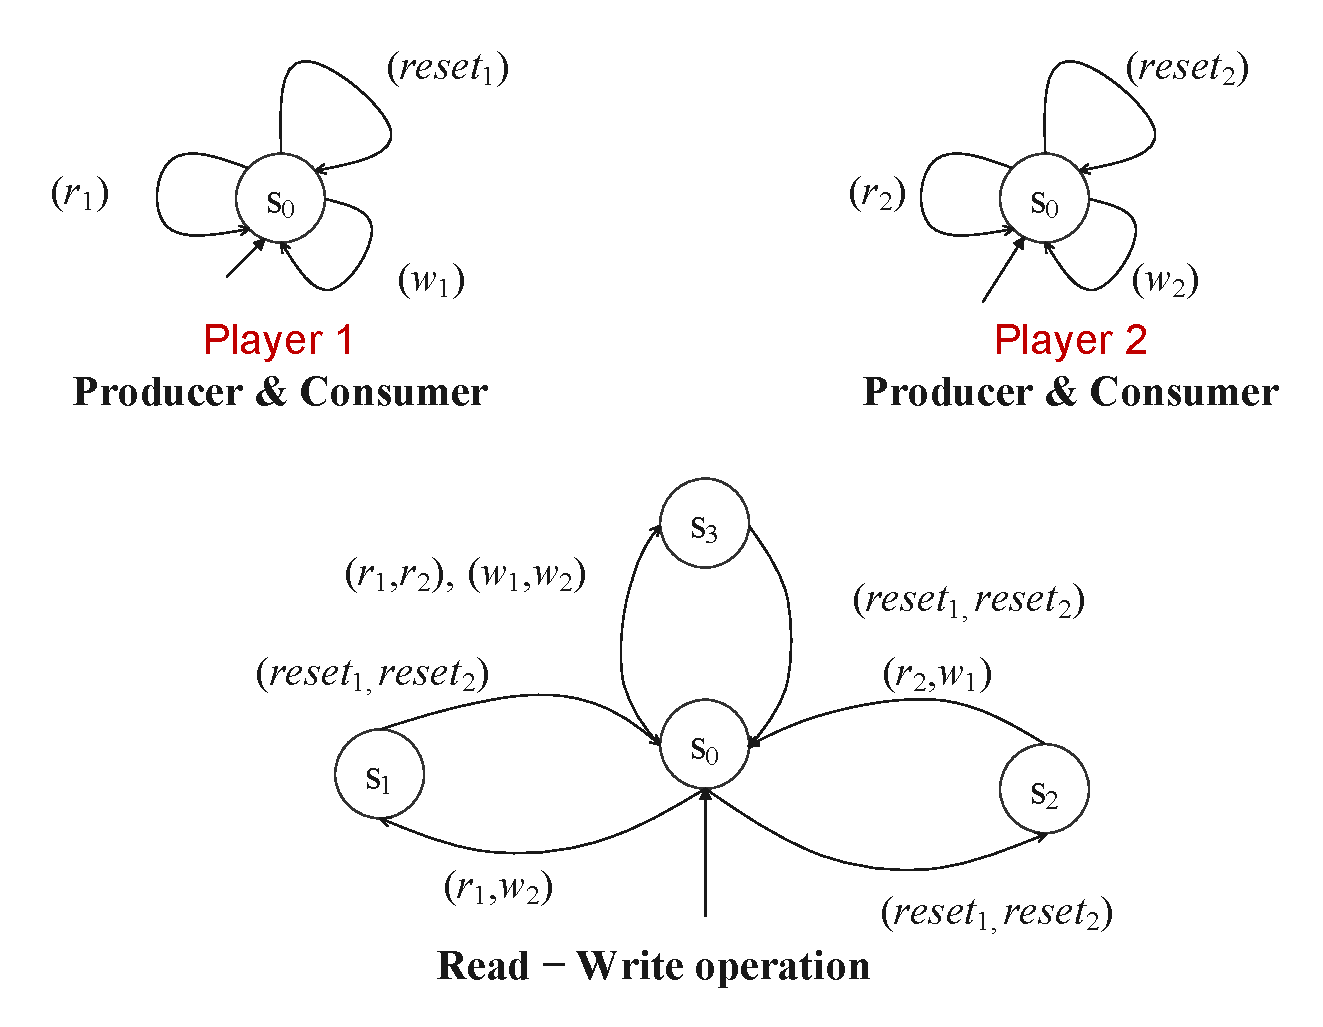
\includegraphics[width=250pt, height =200pt]{examplecsg.pdf}
    \caption{Read and Write Game Model in CSG \cite{BAOUYA2024101161}.}
    \label{fig:even:odds}
\end{figure} 


Considering the modeled system in \fig{fig:even:odds}, when Player 1 initiates the game and emerges victorious by writing, the property is expressed as: \emathtt{\langle\langle 1 \rangle\rangle P_{>0.99}=? [ F \ win=1 ]}. The model and properties associated with the example are available at \cite{BAOUYA2024101161}. 


A dedicated non-player module orchestrates read and write operations in the PRISM code of \lst{exampleinprism}. All commands are labeled with at least two ports, corresponding to the players responsible for triggering the internal write and read operations. The \quot{win} variable defines the player's success in writing (taking values 1 or 2).
The first commands in lines 5-6 represent unscheduled writing (i.e., reading) operations. As these operations are executed, a reset command is introduced in line 8 to indicate an idle state. Subsequently, the commands depicted in lines 9-10 enforce an order between writing and reading operations.  
\lstdefinestyle{framed}
{
	frame=lrb,         
	mathescape,
	numbers=left,
	belowcaptionskip=-1pt,
    xleftmargin=3.11em,
		xrightmargin=0.03cm,
    framexleftmargin=3em,
	framexrightmargin=0pt,
	framextopmargin=5pt,
	framexbottommargin=5pt,
	framesep=0pt,
	rulesep=0pt,
	numbers=left,
}
    
%\lstset{breaklines=true,style=framed,escapeinside={<@}{@>},
%	morekeywords={void, int, public,private,class,protected, submodules, network,connections, const, init,int,,bool, double, module,rewards,endrewards, endmodule},basicstyle=\scriptsize\ttfamily, keywordstyle=\bfseries\color{eminence}, 
%	morecomment=[f][\color{forestgreen}][0]{/*},
%    label=queueemodel
%}
\lstset{
    breaklines=true,
    style=framed,
    escapeinside={<@}{@>},
    morekeywords={void, int, public, private, class, protected, submodules, network, connections, const, init, int, bool, double, module, rewards, endrewards, endmodule},
    basicstyle=\scriptsize\ttfamily,
    keywordstyle=\bfseries\color{blue},
    morecomment=[f][\color{green!70!black}][0]{/*},
        morecomment=[l][\color{green!30!black}]{//},
    label=queueemodel
}


\begin{figure}[!htb]            
\begin{minipage}{9cm}
\begin{lstlisting}[style=framed,%customc,
	caption=PRISM Code for Read/Write of \fig{fig:even:odds},
 	label=exampleinprism]	
module Orchestrator
 win : [0..2]init 0;
 a : [0..2]init 0;
	
 [w1,w2] s=0 -> (s'=1) & (win'=0);
        [r1,r2] s=0 -> (s'=1) & (win'=0);

 [reset1,reset2] s=1 | s=2 | s=3 -> (s'=0) & (win'=0);
 [r1,w2] s=0 -> (s'=2) & (win'=2);
 [w1,r2] s=0 -> (s'=3) & (win'=1);
endmodule
\end{lstlisting}
 \end{minipage}  
\end{figure}

\end{example}